\section{Introduction}
\label{sec:introduction}

  \todo{To complete}

  Nous avons deux objectifs distints, bien que l'un nécessite le second:
  \benumline \item créer des processus distants, c'est à dire mettre le
  processus résultant d'un \texttt{fork()} sur un autre cluster que celui ayant
  fait l'appel et \item migrer des processus existants sur un autre cluster que
  leur cluster actuel\eenumline.

\section{Environnement}
\label{sec:environnement}

  \subsection{TSAR}
  \label{subsec:tsar}

    \todo{To complete}

    TSAR (\textit{Tera-Scale ARchitecture})\cite{tsar} est un projet européen
    MEDEA+ regroupant plusieurs grands acteurs industriels ainsi que des
    laboratoires publics visant à créer une nouvelle architecture matérielle
    permettant le support de plusieurs centaines de coeurs. Ce projet a donné
    naissance à l'architecture TSAR, ainsi qu'à son prototype (TSAR-Leti),
    construit par le CEA.

    La figure \ref{fig:tsar} nous montre un schéma de l'architecture TSAR. Les
    différents processeurs sont regroupés par 4 maximum dans ce que l'on nomme
    un \textbf{cluster}. La mémoire disponible est de 1To, et chaque cluster
    gère son banc mémoire de 4Go. On peut avoir au maximum 4096 processeurs, et
    donc 1024 clusters. Les clusters sont interconnectés entre eux via des NoC
    (\textit{Network on Chip}) DSPIN
    %\cite{dspin}
    . TSAR propose trois niveaux de caches. Chaque processeur dispose de son
    cache L1. On a un cache L2 pour quatre cluster, puis autant de cache L3 que
    de cluster. La cohérence des caches est assurée à 100\% par le matériel via
    le protocole \textbf{DHCCP}
    %\cite{dhccp}
    . Les clusters sont totalement indépendants et n'ont aucune connaissance de
    leur voisins. C'est le système d'exploitation qui va devoir reconnaitre
    l'architecture et gérer les communications entre les clusters.

    \begin{figure}[!h]
      \centering
      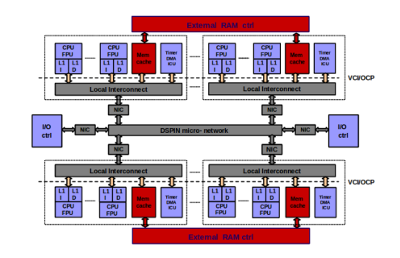
\includegraphics[scale=0.3]{tsar}
      \caption{Schéma de l'architecture TSAR \textit{(source: thèse de Ghassan
          Almaless\cite{almos-phd})}}
      \label{fig:tsar}
    \end{figure}


  \subsection{ALMOS}
  \label{subsec:almos}

    \todo{To complete}

    Le système d'exploitation considéré ici se nomme ALMOS\cite{almos}. C'est un
    noyau développé par l'équipe ALSOC du LIP6, initialement par Ghassan
    Almaless, puis complété par Mohamed Karaoui et Clément TODO. Ce noyau
    expérimental a été concu dans le but de trouver une solution effective aux
    problèmes engendrés par les architectures NUMA massivement multi-coeurs
    (plus d'une centaine de processeurs minimum).

    L'objectif d'ALMOS est d'augmenter de manière significative la localité des
    accès mémoires de manière transparente à l'utilisateur/programmeur, de
    fournir une gestion des ressources distribués, et d'assurer les
    prises de décisions relatives à l'allocation mémoire, le placement de
    processus et l'équilibrage de charge de manière multi-critères et sans
    verrou.

    ALMOS propose une nouvelle vision de la notion de thread. En effet, il a été
    montré que les noyaux actuels (mono/micro-litique, exo-noyau,
    multi-noyau\ldots) ne sont intrinsèquement pas capables d'augmenter la
    localité des accès mémoire. En effet, la notion actuel de thread n'a pas un
    grain assez fin. Dans la structure \texttt{struct task}\footnote{Structure
      représentant un thread dans le noyau Linux}, il n'est jamais fait mention
    des pages physiques accédées. Ainsi, le noyau est incapable de savoir si les
    données relatives à ce thread sont locales au cluster, ou sur un cluster
    distant. ALMOS propose une alternative à ce problème en redéfinissant le
    thread et le procesus et en introduisant les \textbf{processus hybrides}, et
    en introduisant une nouvelle stratégie de répartition mémoire nommée
    \textbf{Auto-Next-Touch}.
